\chapter{Results and Analysis}
\label{details}
This chapter mainly talk about 
\begin{enumerate}
    \item Do the simulation based one computer physics library. Totally, 100 different rigid motion simulation should be finished. For every simulation, fixed steps should be recorded.
    \item Restore information of each state of per simulation by using \textbf{XML} formats, including positions, velocities, contact forces, etc.
    \item Read \textbf{XML} file, and then generate some grid images for training.
    \item Do the deep learning based on training dataset which is created by last step.
    \item Apply the trained model to initialize the values of contact forces($\lambda$). Then compare deep learning method and classical methods.
\end{enumerate}

\section{Rigid Motion Simulation}

\textbf{pybox2d}\footnote{\url{https://github.com/pybox2d/pybox2d}} is chosen as the main physics engine to implemente computer simulation experiments. \textbf{pybox2d} is a 2D physics library for your games and simple simulations. It's based on the Box2D library, written in \textit{C++}. It supports several shape types (circle, polygon, thin line segments), and quite a few joint types (revolute, prismatic, wheel, etc.). 

\subsection{Simulation Configuration}
    \label{simconfig}
    \begin{itemize}
        \item \textbf{World Setting}, the world box size is $30\times30$,   and there are $100$ circle rigids($r=1$, all circle rigid bodies in the same size.) inside the box. Initially, the rigid circles will be located following gaussian distribution\footnote{\url{https://en.wikipedia.org/wiki/Normal_distribution}}. Then, all rigid circles will fall down by gravity. The visualization of simulation is shown in Figure \ref{fig:imsim}.
        \item \textbf{Simulation Setting}, there will be totally $600$-steps simulation. For each step, $\Delta t = 0.01s$, and the number of iteration in  eacg step will be set as fixed, $3000$. Then I will use the average covergence rate to show how fast the model coverages.
    \end{itemize}
\subsection{Simulation Details}
    Before generating data, one dynamic simulation was run to check how \textit{pybox2d} works and some figures have been obtained. Figure \ref{fig:contactnum} describe the relationship between time step and contacts number, and Figure \ref{fig:contacttime} gives the relationship between time spend and contacts number.
    \begin{figure}[!h]
        \centering
        \begin{subfigure}[b]{0.3\textwidth}
            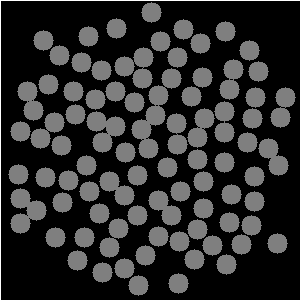
\includegraphics[width=\textwidth]{Figures/sim0.png}
            \caption{Time Step=$0$}
        \end{subfigure}
        \begin{subfigure}[b]{0.3\textwidth}
            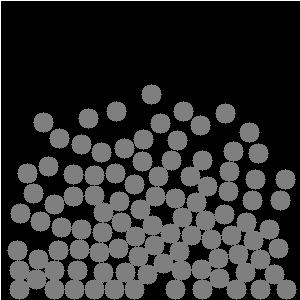
\includegraphics[width=\textwidth]{Figures/sim2.png}
            \caption{Time Step=$200$}
        \end{subfigure}
        \begin{subfigure}[b]{0.3\textwidth}
            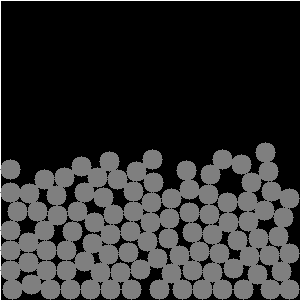
\includegraphics[width=\textwidth]{Figures/sim3.png}
            \caption{Time Step=$400$}
        \end{subfigure}
        \caption{Visualization for experiment simulation}
        \label{fig:imsim}
    \end{figure}
    \begin{figure}[!ht]
        \centering
        \begin{subfigure}[b]{0.7\textwidth}
            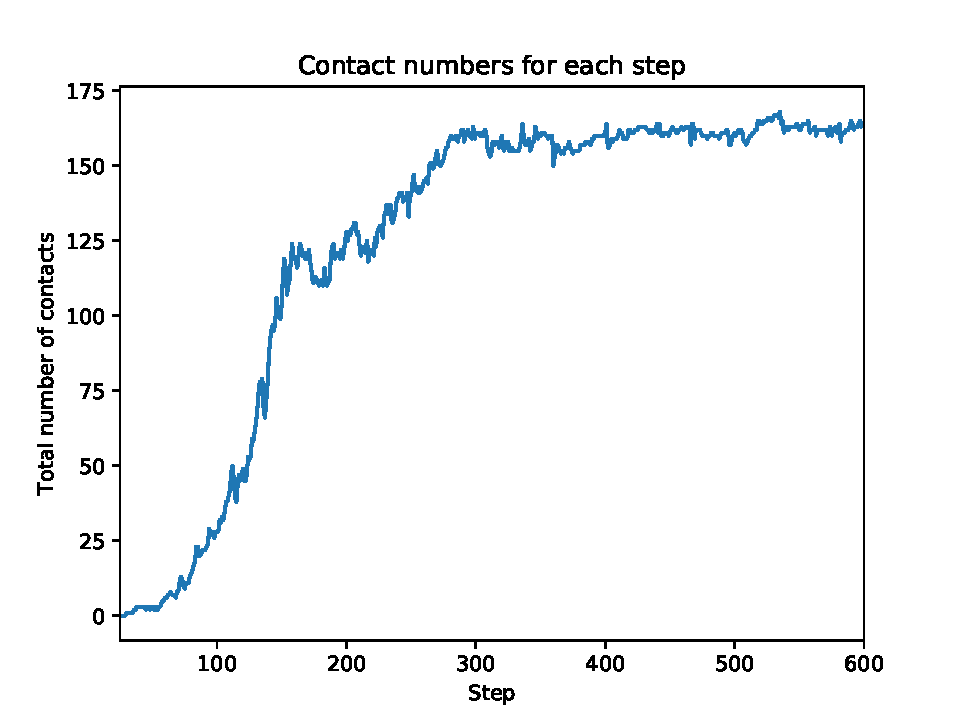
\includegraphics[width=\textwidth]{Figures/contact_num}
            \caption{The number of contacts in each step.}
            \label{fig:contactnum}
        \end{subfigure}
        \begin{subfigure}[b]{0.7\textwidth}
            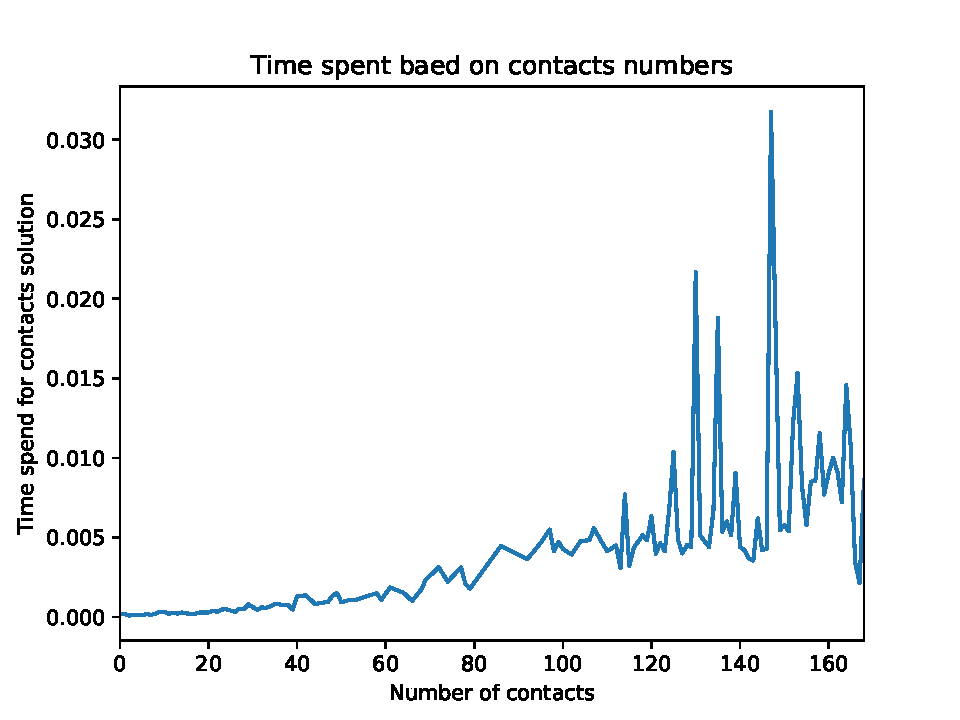
\includegraphics[width=\textwidth]{Figures/contact_time}
            \caption{Time spend for contact solution.}
            \label{fig:contacttime}
        \end{subfigure}
        \caption{Visualization for experiment simulation}
    \end{figure}

\subsection{SPH parameters}
    \label{SPH-setting}
    In Section \ref{SPHtest}, it has been tested that \textbf{SPH} is a good strategy to generate grid images representing a discrere snapshot of the dynamics. Then, the grid size and smoothing length $h$ are import to our data generation. The grid size should be reasonable so that there is no two contact points are mapped into the same cell, since if there are more than two contact values in one cell, it will be hard for CNN to recognize, which will decrease the accuracy of prediction. This was mentioned in section \ref{gs}.
    \begin{figure}[!h]
        \centering
        \includegraphics[width=0.4\textwidth]{Figures/SPHvi.pdf}
        \caption{Example visiualization for Smoothed Particle Hydrodynamics. The small red circles stand for the grid nodes, and the blue circles stand for kernel size.}
    \end{figure}

    \subsubsection{Grid Size and Kernel Length}
    I define $\pmb{d}=(d_x, d_y)$ as grid cell size and $h$ as smoothing length. I conclude some rules for determining grid cell size and smoothing length. 
    \begin{itemize}
        \item Since the objects are circles, the ideal cell size should like,
            $$d_x = d_y = d $$ 
        \item Since there can not be two contact points are mapped into the same cell, $d$ must be less than the distance of nearest two contact points. It can be defined.
            $$d \le r = 1$$
        \item Similarly, if one contact point can only be mapped to one cell, the smooth length $h$ should be less than the minimum distance between two contact points $d$,
            $$h \le d$$  
        \item For a given $d$, whatever the contact position $\pmb{q}=(q_x, q_y)$ is, its information can be restore in nearby nodes. So it can be,
            $$h \ge \frac{\sqrt{2}}{2}d \approx 0.71 d$$
    \end{itemize}
    One experiment has been designed to test whether the rules can be applied in this case. Still using the simulation config introduced in section \ref{simconfig}. The cell size is fixed, $d=0.25$. Different smoothing length is appiled. The results are shown in Figure \ref{fig:dh}. \\

    As what is shown in Figure \ref{fig:dh}, when $h=0.4d$ or $h=2d$, the solver coverages more slowly and unstable. Overall, for the next step, data generation, I will make $h=d$ always. The next step is to explore what $d$ value will be good.
    \begin{figure}[!ht]
        \centering
        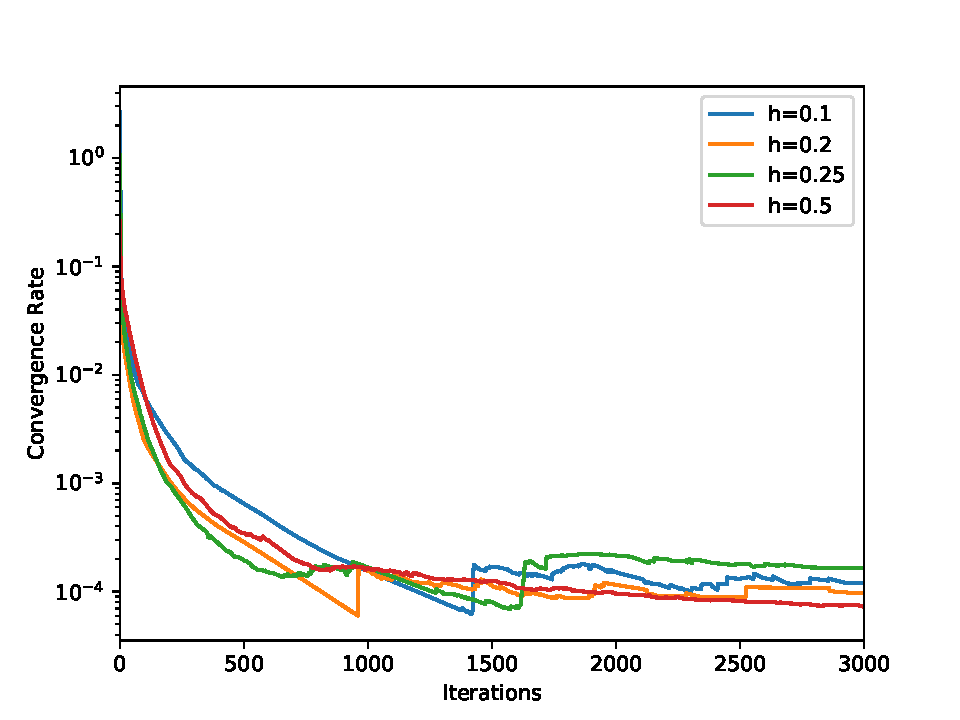
\includegraphics[width=0.7\textwidth]{Figures/size25.pdf}
        \caption{The grid size $d$ is set $0.25$. $h=0.1, 0.2, 0.25, 0.5$ is tested respectively. This figure shows different coveragence rate based on different $h$ value.}
        \label{fig:dh}
    \end{figure}
    $h=d$ has been determined, the next step is to choose the value of $d$. Another experiment is taken to check the convergence rate with using diffrent $d$ values. The reults are showns in Figure \ref{fig:testd}. From this figure, it is obviously, when $d=0.5$, iterative solver converages the most rapidly. 
    \begin{figure}[!ht]
        \centering
        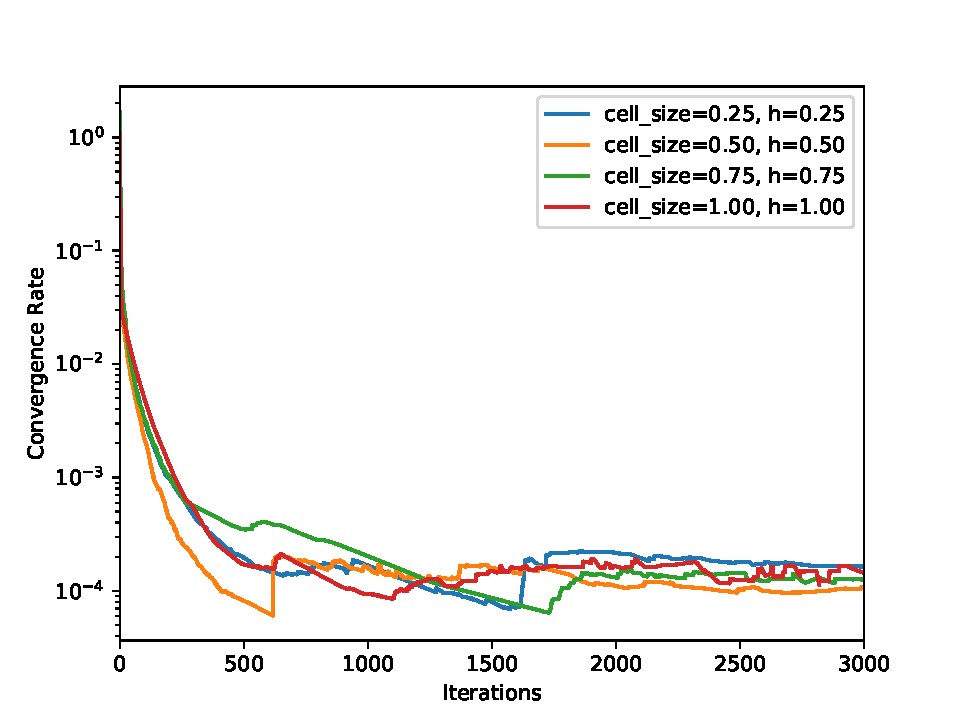
\includegraphics[width=0.7\textwidth]{Figures/hd.pdf}
        \caption{Coveragence rate for different $d$ value.}
        \label{fig:testd}
    \end{figure}
    \textbf{Importantly}, $d=0.5~~\text{and}~~h=0.5$ is not always the best experimented with different numbers of rigid inside the world box. But, it generally performs better than other values. As a result, I will choose $h=d=0.5$ as the parameters for SPH method.
    $$d_x = d_y = 0.5~~\text{and}~~h=0.5$$
    \subsubsection{Kernel Choosing}
    The choice of kernel also needs to be addressed. In the paper, two kernels, \textbf{Poly6} and \textbf{Spiky}, have been introduced in section \ref{sec:kernels}. These two kernels are seperately used based on Algorithm \ref{testSPH}. Then, the plot about coveragence rate of different kernels is obtained. From the plot, it is clear that kernel \textbf{Poly6} perform better.  
    \begin{figure}[!ht]{}
        \centering
        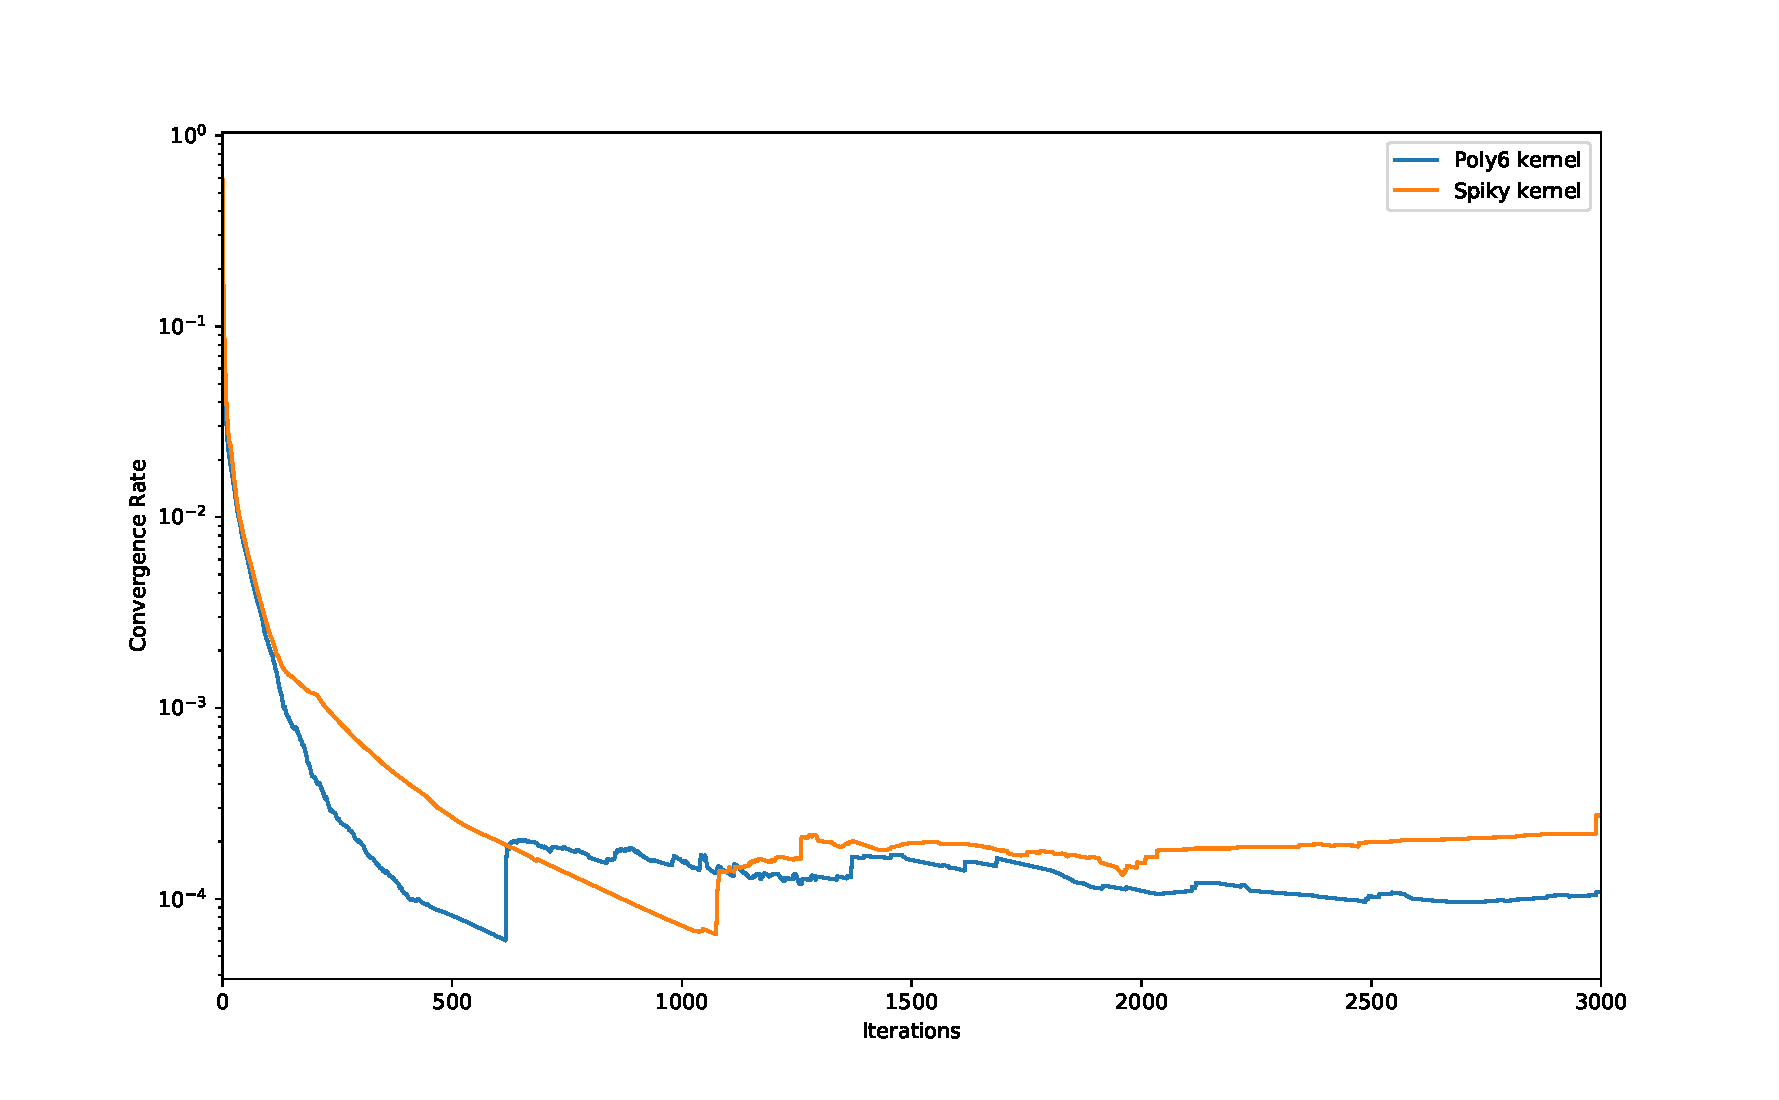
\includegraphics[width=0.8\textwidth]{Figures/kerneltest.pdf}
        \caption{Coveragence rate for kernel \textbf{Poly6} anf \textbf{Spiky}}
        \label{fig:testd}
    \end{figure}
    As a conclusion, SPH with \textbf{Poly6} kernel($\pmb{d} = (0.5, 0.5)$, smoothing length $h=0.5$), will be used for particle-grid transformation. \\

    After determining grid size and smoothing length, I will compare this specific \textbf{SPH-Model} with other models mentionde in section \ref{SPHtest}, following Algorithm \ref{testSPH}. The result is shown in Figure \ref{fig:final_test}.
     \begin{figure}[!ht]
        \centering
        \includegraphics[width=0.8\textwidth]{Figures/final_SPH.pdf}
        \caption{Coveragence rate for models(different initial values for $\pmb{\lambda}$).}
        \label{fig:final_test}
    \end{figure}
    Unlike the result shown in Figure \ref{fg:addSPH}. Compared with other models, \textbf{SPH-Model} gets convergence much faster. So, $h=d=0.5$ is a good choice for this project and the future steps.

\section{Data Generation}
To create data that are more accessible to learning, I will map a discrete element method into a continuum settig use techniques from smooth particle hydrodynamics(SPH). In order to get enough avaliable training data and remove useless information, I used
\begin{itemize}
    \item $150$ simulation with different initial configuration. The number of circle objects is not fixed as well. However, if there is too few objects inside the box, contacts might not happen until the simulation ends up. So the number of objects will be in range of $[70, 110]$.
    \item If there is no contact in one state, the state means nothing to the learning. So the states without any contacts will be removed.
\end{itemize}

\subsection{XML Restoration}
In each simulation, state in every time step will be stored in one \textbf{xml} file. The structure of the body is consist of \textbf{mass}, \textbf{position}, \textbf{velocity}, \textbf{spin omega} and \textbf{inertia}. The structure of contact is consist of \textbf{postion}, \textbf{impulse}(including in normal direction and tangent direcrion), \textbf{master} body and \textbf{slave} body. Two examples are given in the following.\\

This is nn example for one body information is given below.
\begin{lstlisting}[language=XML]
    <body index="86" type="free">
        <mass value="3.14159274101"/>
        <position x="7.79289388657" y="2.62924313545"/>
        <velocity x="2.7878344059" y="-1.45545887947"/>
        <orientation theta="-0.115291565657"/>
        <inertia value="1.57079637051"/>
        <spin omega="-2.33787894249"/>
        <shape value="circle"/>
    </body>
    ...
\end{lstlisting}
Another example \textit{XML} code is for contatc force.
\begin{lstlisting}[language=XML]
    <contact index="1" master="2" master_shape="b2CircleShape(childCount=1, pos=b2Vec2(0,0), radius=1.2000000476837158, type=0,)" slave="97" slave_shape="b2CircleShape(childCount=1, pos=b2Vec2(0,0), radius=1.2000000476837158, type=0, )">
        <position x="0.21963849663734436" y="13.875240325927734"/>
        <normal normal="b2Vec2(-1,2.9819e-05)"/>
        <impulse n="0.005236322991549969" t="-0.002184529323130846"/>
    </contact>
    ...
\end{lstlisting}

\subsection{SPH configuration}
As it is talked in \ref{SPH-setting}, 
\begin{itemize}
    \item \textbf{Kernel}, Poly6, which you can see in section \ref{poly6}.
    \item \textbf{Kernel Settings}, cell size $d_x=d_y=0.5$, smoothing length $h=0.5$.
\end{itemize}
\subsection{XML to grid}
After getting a set of \textbf{xml} file, the next step is to read state information from \textbf{xml} file, and then map them to grid images with SPH based method. The channel of each image will be 8, including $[m, v_x, v_y, \omega, n_x, n_y, \lambda_n, \lambda_t]$. Since $n_y$ is related to $n_x$, I remove $n_x$ from the channels. \\

For the learning, I devide 8 channels to features(input) and label(output).
    $$\text{Feature} = [m, v_x, v_y, \omega, n_x]$$
    $$\text{Label} = [\lambda_n, \lambda_t]$$



\section{CNN Training}
\subsection{CNN  Architecture}
    The neural network was designed using Keras\cite{chollet2015keras}. Keras is a neural networks Application Programming Interface (API) written in Python, it runs on top of either TensorFlow. With some inspiration from AlexNet\cite{Krizhevsky:2012:ICD:2999134.2999257}, the networks shows five constracting stacks of layers and each stack is consist of two or three convolutional layers in the same size. To avoid overfitting, each stack is followed by one dropout layer. One full-connected layer is set after the last convolutional layer. This input layer is followed by a batch normalization layer, normalizing images within a batch, which is discussed in section \ref{batchnor}. This architecture includes $64,498,866$ weights for an input size of ($41\times41\times5$). All convolutional layers have kernels of size $(3\times 3\times d)$, and are followed by ReLU activation function. Figure \ref{fig:art} shows visualization of model architecture, and Table \ref{table:layers} shows the specific information about parameters when input images go through the CNN.

    \begin{figure}[!h]
        \centering
        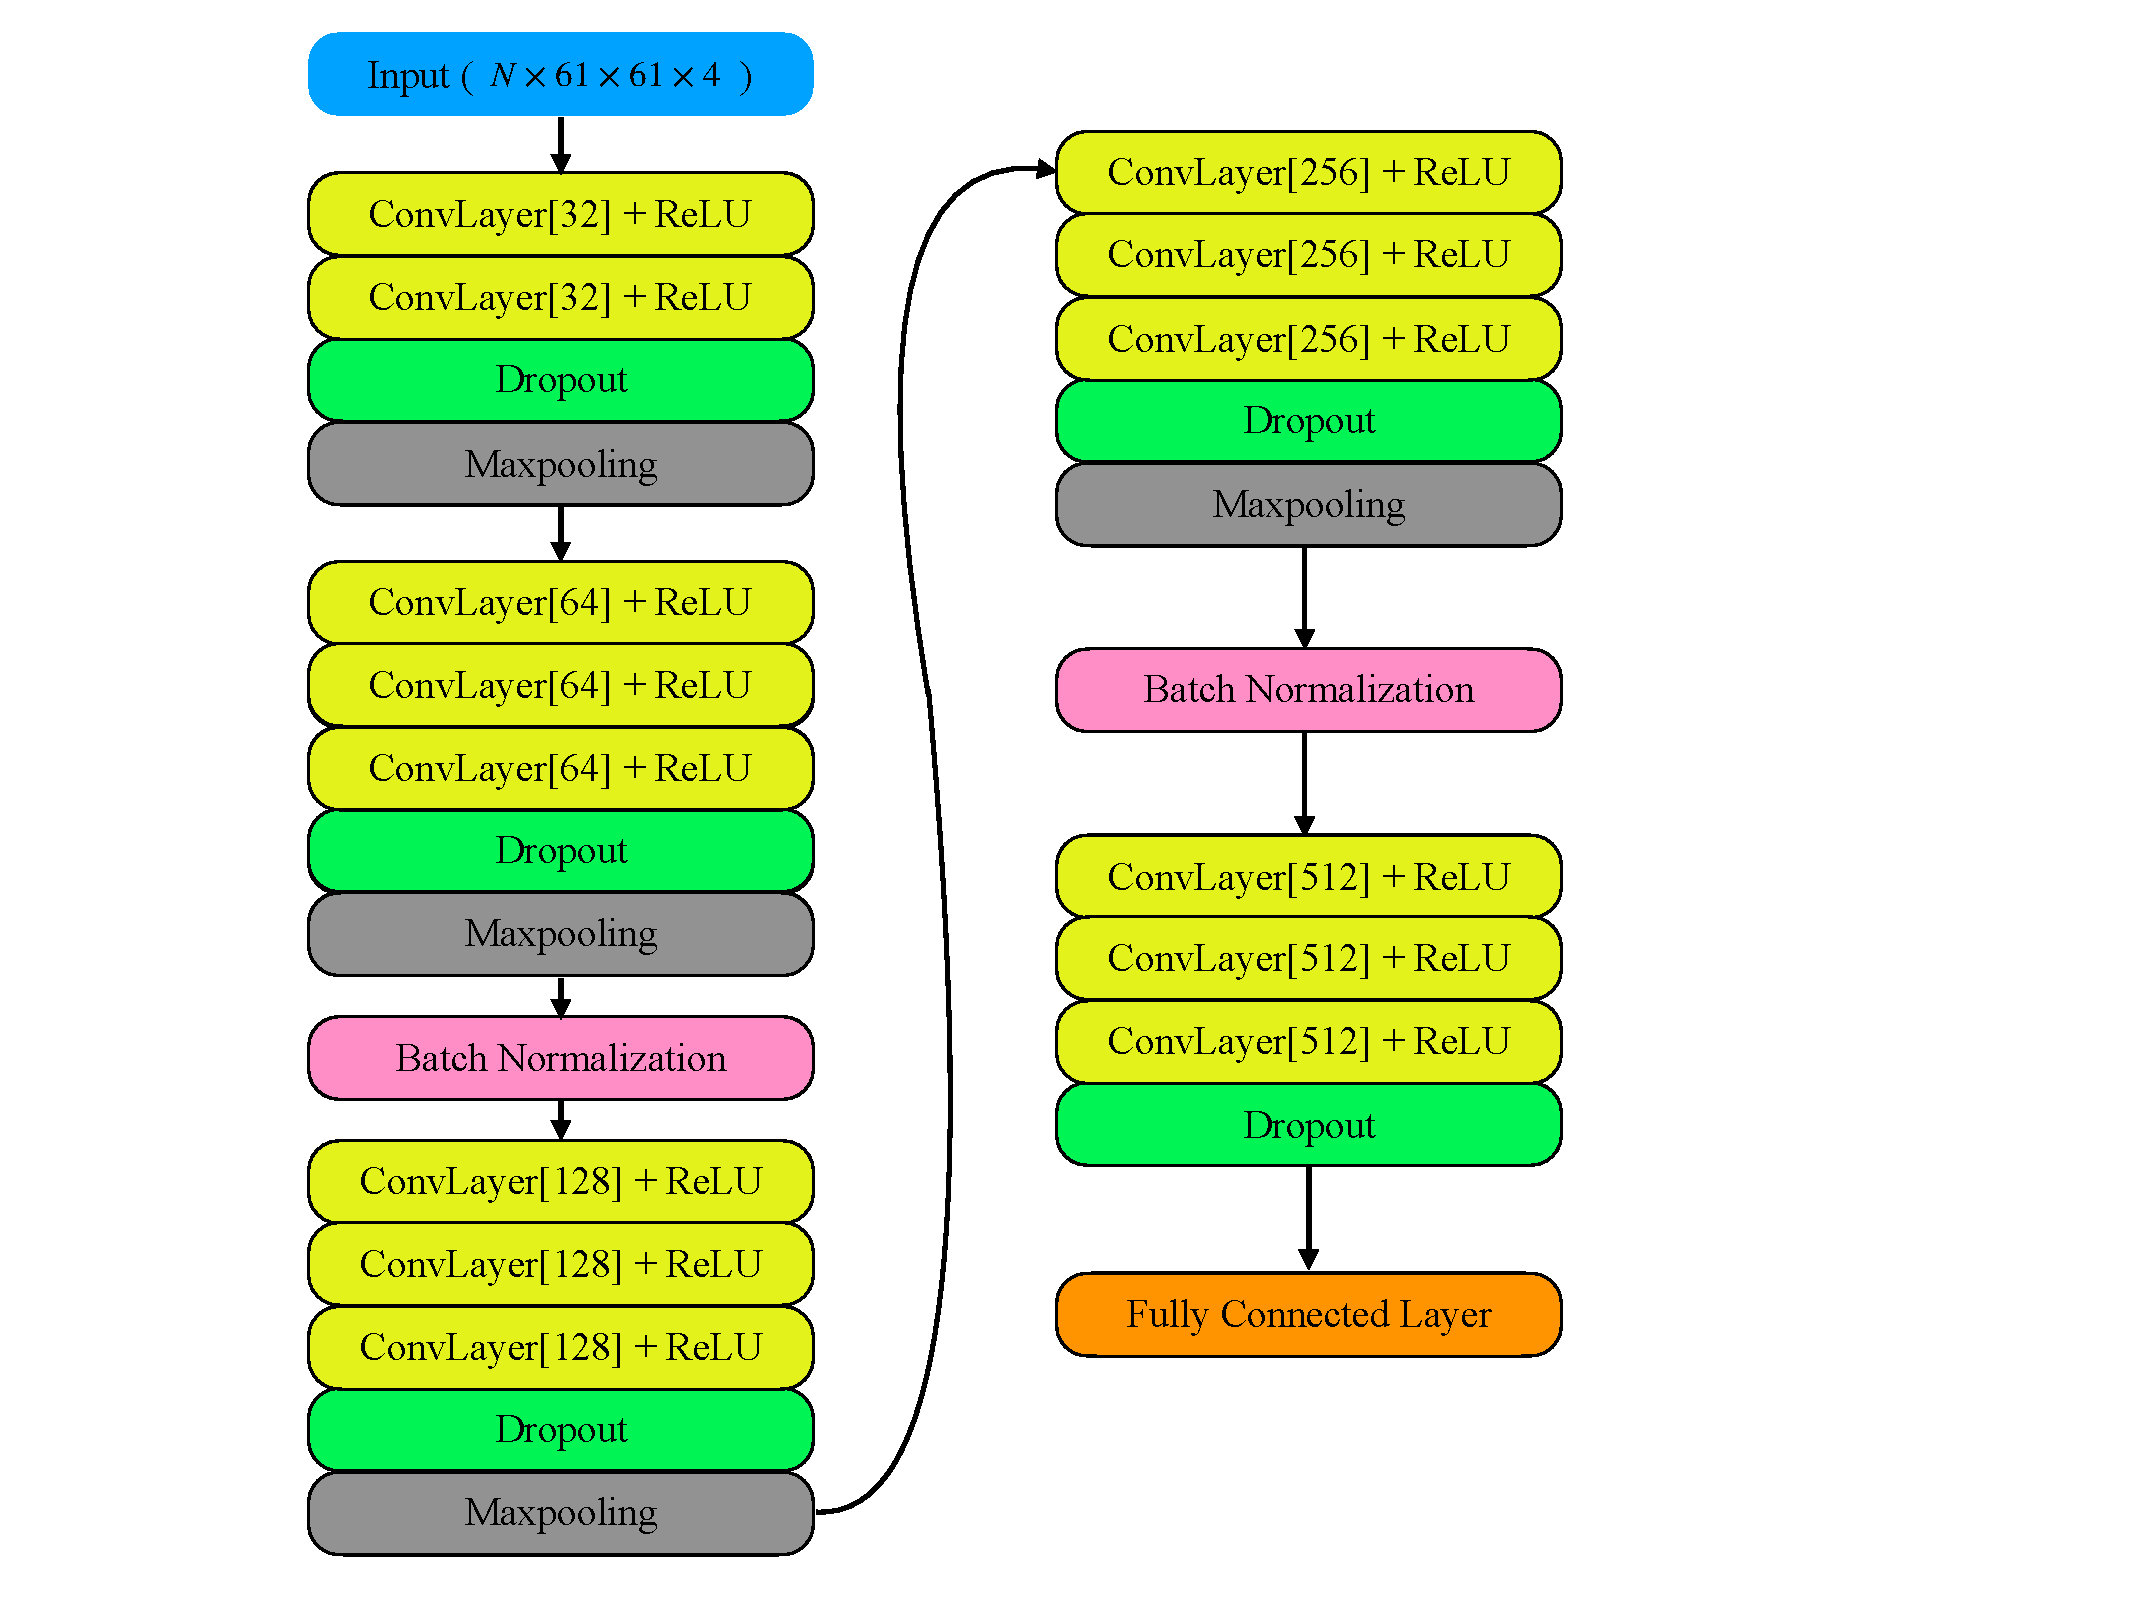
\includegraphics[width=\textwidth]{Figures/cnn_arc.pdf}
        \caption{Architecture of CNN model}
        \label{fig:art}
    \end{figure}

    \begin{table}[h!]
        \centering
        \begin{tabular}{ l | c  }
            Layer & Output Shape  \\ \hline
            Input & $n_b\times61\times61\times5$  \\
            Convolution(32) & $n_b\times61\times61\times32$  \\
            Convolution(32) & $n_b\times61\times61\times32$  \\
            Dropout & $n_b\times61\times61\times32$  \\
            MaxPooling & $n_b\times31\times31\times32$ \\
            Convolution(64) & $n_b\times31\times31\times64$  \\
            Convolution(64) & $n_b\times31\times31\times64$  \\
            Convolution(64) & $n_b\times31\times31\times64$  \\
            Dropout & $n_b\times31\times31\times64$  \\
            MaxPooling & $n_b\times16\times16\times64$ \\
            BatchNormalization & $n_b\times16\times16\times64$ \\
            Convolution(128) & $n_b\times16\times16\times128$  \\
            Convolution(128) & $n_b\times16\times16\times128$  \\
            Convolution(128) & $n_b\times16\times16\times128$  \\
            Dropout & $n_b\times16\times16\times128$  \\
            MaxPooling & $n_b\times8\times8\times128$ \\
            Convolution(256) & $n_b\times8\times8\times256$  \\
            Convolution(256) & $n_b\times8\times8\times256$  \\
            Convolution(256) & $n_b\times8\times8\times256$  \\
            Dropout & $n_b\times8\times8\times256$  \\
            MaxPooling & $n_b\times4\times4\times256$ \\
            BatchNormalization & $n_b\times4\times4\times512$  \\
            Convolution(512) & $n_b\times4\times4\times512$  \\
            Convolution(512) & $n_b\times4\times4\times512$  \\
            Convolution(512) & $n_b\times4\times4\times512$  \\
            Dropout & $n_b\times4\times4\times512$ \\
            Flatten & $n_b\times8192$ \\
            Dense & $n_b\times7442$ \\    
        \end{tabular}
        \caption{Feature map (tensor) sizes through the network, the input has size $n_b\times61\times61\times5$, with batch size $n_b$ and patches of size $61\times61\times5$.}
        \label{table:layers}
    \end{table}

\subsection{Traing Configuration}
\subsubsection{Loss Function}
Firstly, we define a filter funtion,
\begin{equation}
    g(x)= \begin{cases} 0, \quad x = 0 \\ 1, \quad x \ne 0 \end{cases}
\end{equation}
Then, we can update the loss function based on Euqation \ref{eq:mse}. 

\begin{equation}
    L = \frac{1}{N}\sum_{i}^{N}g(\hat{y}_i)(y_i-\hat{y}_i)^2
\end{equation}

\subsection{Training Details}
    The learning happened on GPU(\textit{GeForce GTX 1080 Ti, 11 Gbps GDDR5X memory})\footnote{\url{https://www.nvidia.com/en-us/geforce/products/10series/geforce-gtx-1080-ti/}} held by Image Section, DIKU\footnote{\url{https://di.ku.dk/english/research/imagesection/}}. The whole learning takes nearly 24 hours. The model you can download in my personal dropbox\footnote{\url{https://www.dropbox.com/s/jrwzqib6ghrq59i/model.h5?dl=0}}. I gave hyperparameters setting below,
    \begin{table}[h!]
        \centering
        \begin{tabular}{ l | c  }
            Hyperparameter  & Setting \\ \hline
            Activation function & ReLU \\
            Weight initilization & He normal\cite{sutskever2013importance} \\
            Weight regularizer &  L2 \cite{hinton2006fast} \\
            Convolution border mode   & Same \\
            Stride & 2 \\ 
            Kernel size & $(3, 3)$ \\
            Dropout rate & $0.1$ \\
            Optimizer & SGD \\
            Initial Learning Rate & $1\times 5\times10^{-3}$ \\
            Batch Size & 200 \\
            Epoch & 1000 \\
            Validation Rate & 0.2 \\
        \end{tabular}
        \caption{Hyperparameter settings.}
        \label{table:hyper}
    \end{table}
    \subsubsection{Learning Rate}
    The learning rate will change with the number of epoch, as talked in section \ref{learning}. I will give a specific value as the learning rate depending on the number of epoch. The learning rate will become smaller with increasing epoch. 
    data. The overall algorithm is concluded in Algorithm \ref{ls}.
    \begin{algorithm}[!h]
        \KwData{$epoch$}
        \KwResult{learning rate $\eta$}
        \If {$epoch < 100$}{$\eta = 5\times10{-3}$}
        \If {$100< epoch < 300$}{$\eta = 2\times10^{-3}$}
        \If {$300< epoch < 500$}{$\eta = 1\times10^{-3}$}
        \If {$epoch > 300$}{$\eta = 2\times10^{-4}$}
        \caption{Learning Rate Scheduling}{}
        \label{ls}
    \end{algorithm}


\section{Simualtion based on Trained Model}
Once getting the trained model, the next step is to apply this model in simulation based on Algorithm \ref{al:basic} and compare it with other solutions.\\

I applied it in one test world built by the setting mentioned in section \ref{simconfig}. The test world is consist one $30 \times 30 $ box and $K$($50<K<100$) randomly distributing balls($r=1$). The balls will fall down due to gravity. Figure \ref{testoneworld} shows the details. As what is expeted, CNN model performs similar with \textbf{SPH-Model}(mentioned in section \ref{SPHtest}). Although the model is not as good as \textbf{SPH-model}, its coverages rate is obviously faster than buit-in ones. 
\begin{figure}
    \centering
    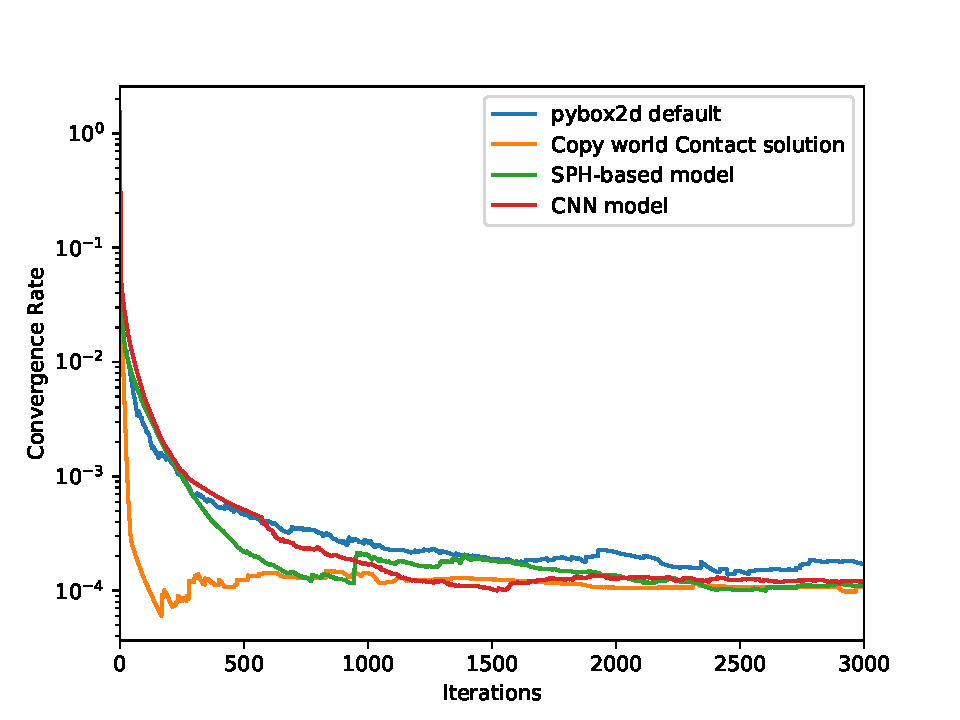
\includegraphics[width=0.8\textwidth]{Figures/same_world.pdf}
    \caption{}
    \label{testoneworld}
\end{figure}
